\documentclass{../source/Experiment}

\major{信息工程}
\name{姚桂涛}
\title{多路竞赛抢答器}
\stuid{3190105597}
\college{信息与电子工程学院}
\date{\today}
\lab{东4-216}
\course{电子电路系统综合实验}
\instructor{李锡华、施红军}
\grades{}
\expname{多路竞赛抢答器设计}
\exptype{设计综合实验}
\partner{杜秉哲、郭含蕾}
\begin{document}
    \makecover
    \makeheader
        在许多比赛活动中,为了准确、公正、直观地判断出第一个抢答者,通常设置一台抢答器,通过数显、灯光及音响等多种手段指示出第一抢答者。此外,还可以设置计分、犯规、限时等功能。在比赛进行时,需要反应及时准确、显示清晰方便的定时抢答器设备。通常有多组参加竞赛,所以抢答器应该包括一个总控制台和多个具有显示及抢答功能的终端。
    \section{设计任务}
        以中规模数字集成电路为核心,设计一台多路竞赛抢答器,要求具有如下功能。

        1.可同时提供8名选手参加比赛,按钮和显示的参赛组编号为1、2、……、8。

        2.主持人有一个控制开关,用来控制系统的复位清零和启动。

        3.抢答器具有数据锁存和组号显示功能。在主持人将系统复位后,组号显示为“0”或不显示;在主持人按下“开始”键后,系统发出短促的“嘀”的提示音,这时参赛者可按抢答按钮进行抢答,最先按动按钮的那组指示绿灯亮,系统发出“嘀-嘟”的双音提示音,同时显示器显示出抢答者的组号。此时系统具有自锁功能,锁存抢答者的输入信息,同时封锁其他抢答者的随后抢答,使随后的其他各组的抢答无效。

        4.定时抢答功能。当主持人按下“开始”钮后,定时器开始以秒减计数并显示剩余时间,参赛者在设定的时间内进行抢答,一旦有选手抢答,定时器立即停止计数。如果定时时间到时还无人抢答,系统发出持续1秒的提示音,定时器停在О秒,本次抢答无效,封锁抢答输入电路,禁止参赛者超时后抢答。抢答的时间可在1-~99秒内由主持人预设。

        5.选做项。判断提前抢答(违规)电路。在主持人启动“开始”钮前,如果有人提前按下抢答按钮,则该组指示红灯亮,并显示出抢答者的组号,系统发出短暂的“嘟”警告音,同时封锁抢答输入电路,本次抢答无效。

        6.选做项。记分电路。每组在开始时预置100分,抢答后有主持人控制,答对加10分,答错减10分。
    \section{方案设计思路}
        1.鉴别第一抢答者。设计任务是要准确判断出第一个抢答者的信号,并将其锁存和显示,同时封锁随后的抢答信号。实现这一功能可用触发器或锁存器,在得到第一信号后立即将电路的输入封锁,阻止随后的抢答信号进入。

        2.当电路获得第一抢答信号后,用绿色LED指示灯指示该组抢答成功,用数码显示电路显示抢答者的组号。同时启动音频电路,使其发出“嘀-嘟”的双音提示音。

        3.抢答定时器。可用时钟专用芯片产生一个标准秒信号,2位可预置数的十进制减法计数器作倒计时定时器。当得到有效的第一抢答信号后停止计数。如果计数器减到О时还未收到有效的第一抢答信号,则同样停止计数,并封锁抢答器,本次抢答无效。同时发出持续1秒的告警提示音。

        4.记分电路可采用2位十进制计数器及数码显示器来实现。由于每次都是加(减)10分,个位数始终为0,所以只要对十位和百位进行加(减)计数即可,个位仅用数码管显示0。
    \section{系统设计}
        \subsection{设计原理}
            基于以上的分析可知,多路竞赛抢答器由抢答输入电路、锁存显示电路、定时电路、声音告警电路及控制电路等组成,可画出抢答器的组成框图如图1,其工作过程为:接通电源后,主持人按下“复位”键,抢答器清零复位,并处于禁止工作状态。在按下“开始”键后,抢答器处于工作状态,系统发出短暂的“嘀”提示音,倒计时定时器工作。当参赛选手按下抢答键时,控制器接收并锁存第一个抢答信号,点亮按钮旁的绿色指示灯,并发出抢答成功的提示音,同时对抢答输入电路进行封锁,禁止其他选手再抢答。编译码及显示电路显示出抢答者的组号。如果有人先于主持人按下“开始”键抢答,控制器则点亮抢答者按钮旁的红色指示灯,并发出告警提示音,显示违规抢答者的组号,同时对抢答输入电路s进行封锁,木次拾答无效。主持人可对得分讲行加(减)控制。
            \begin{figure}[H]
                \centering
                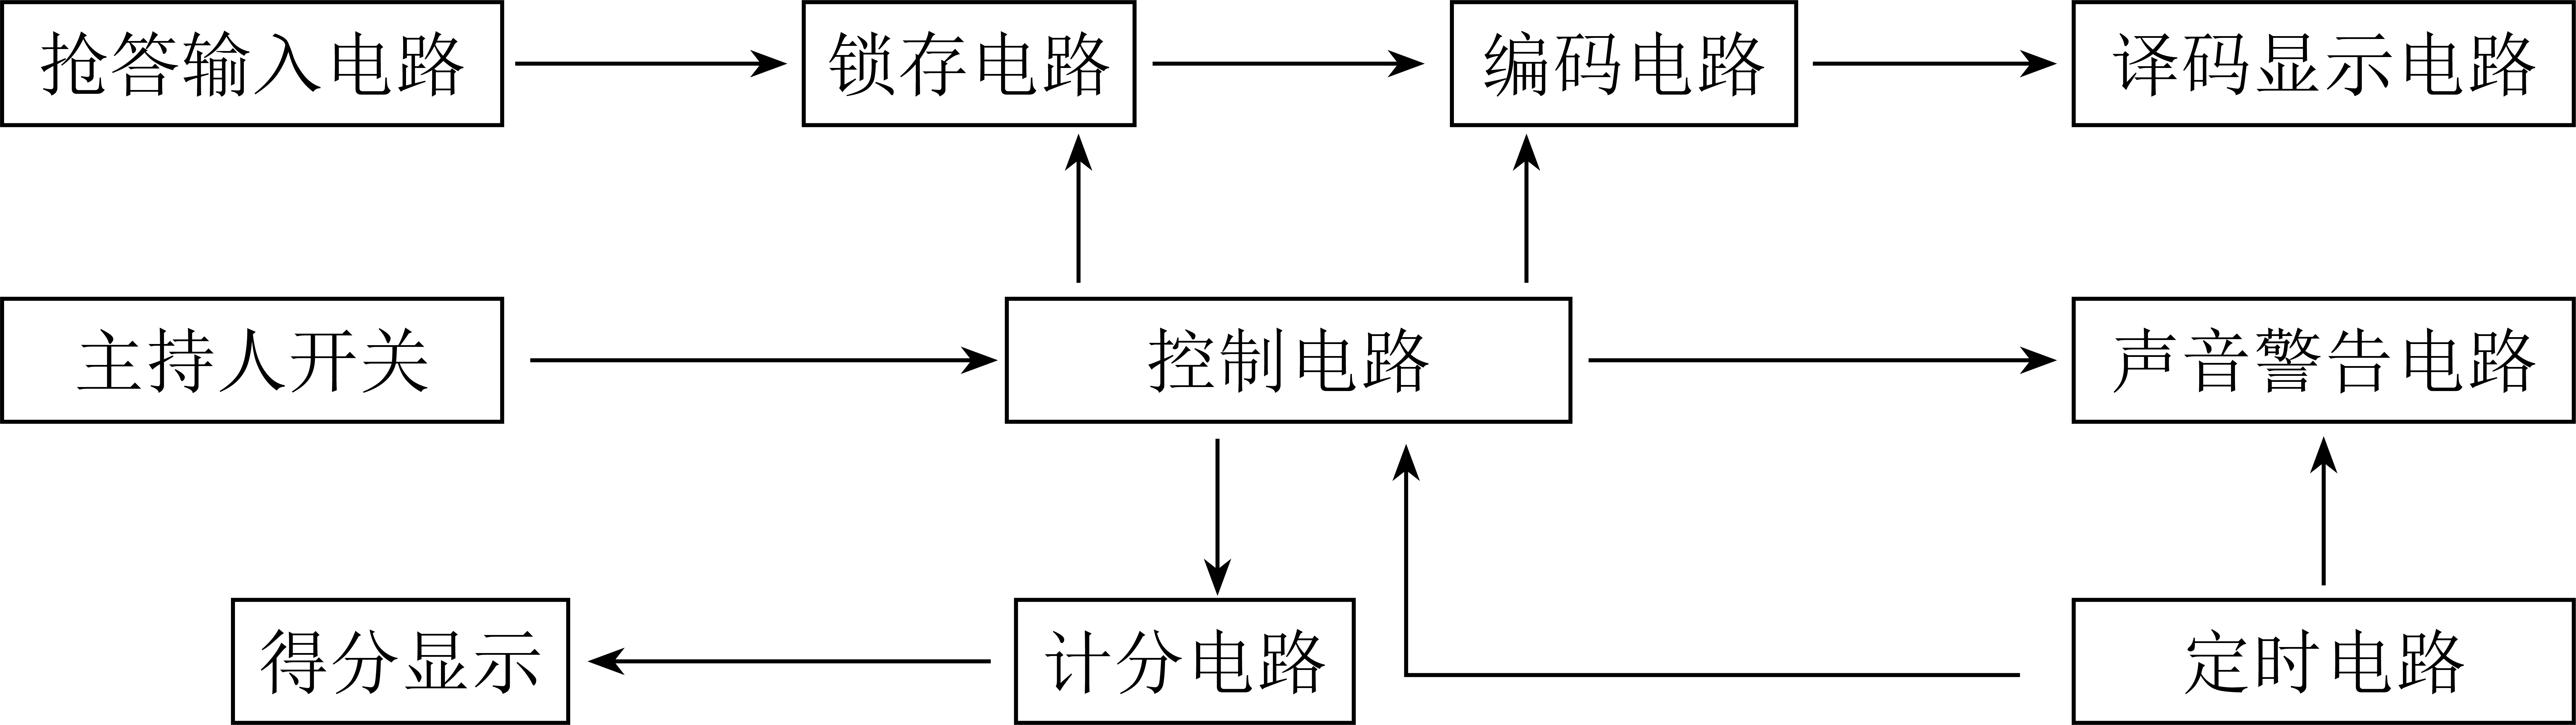
\includegraphics[width = 0.7\textwidth]{pic/思路.png}
                \caption{多路竞赛抢答器电路组成框图}
            \end{figure}
        \subsection{抢答输入电路设计}
            \begin{figure}[H]
                \centering
                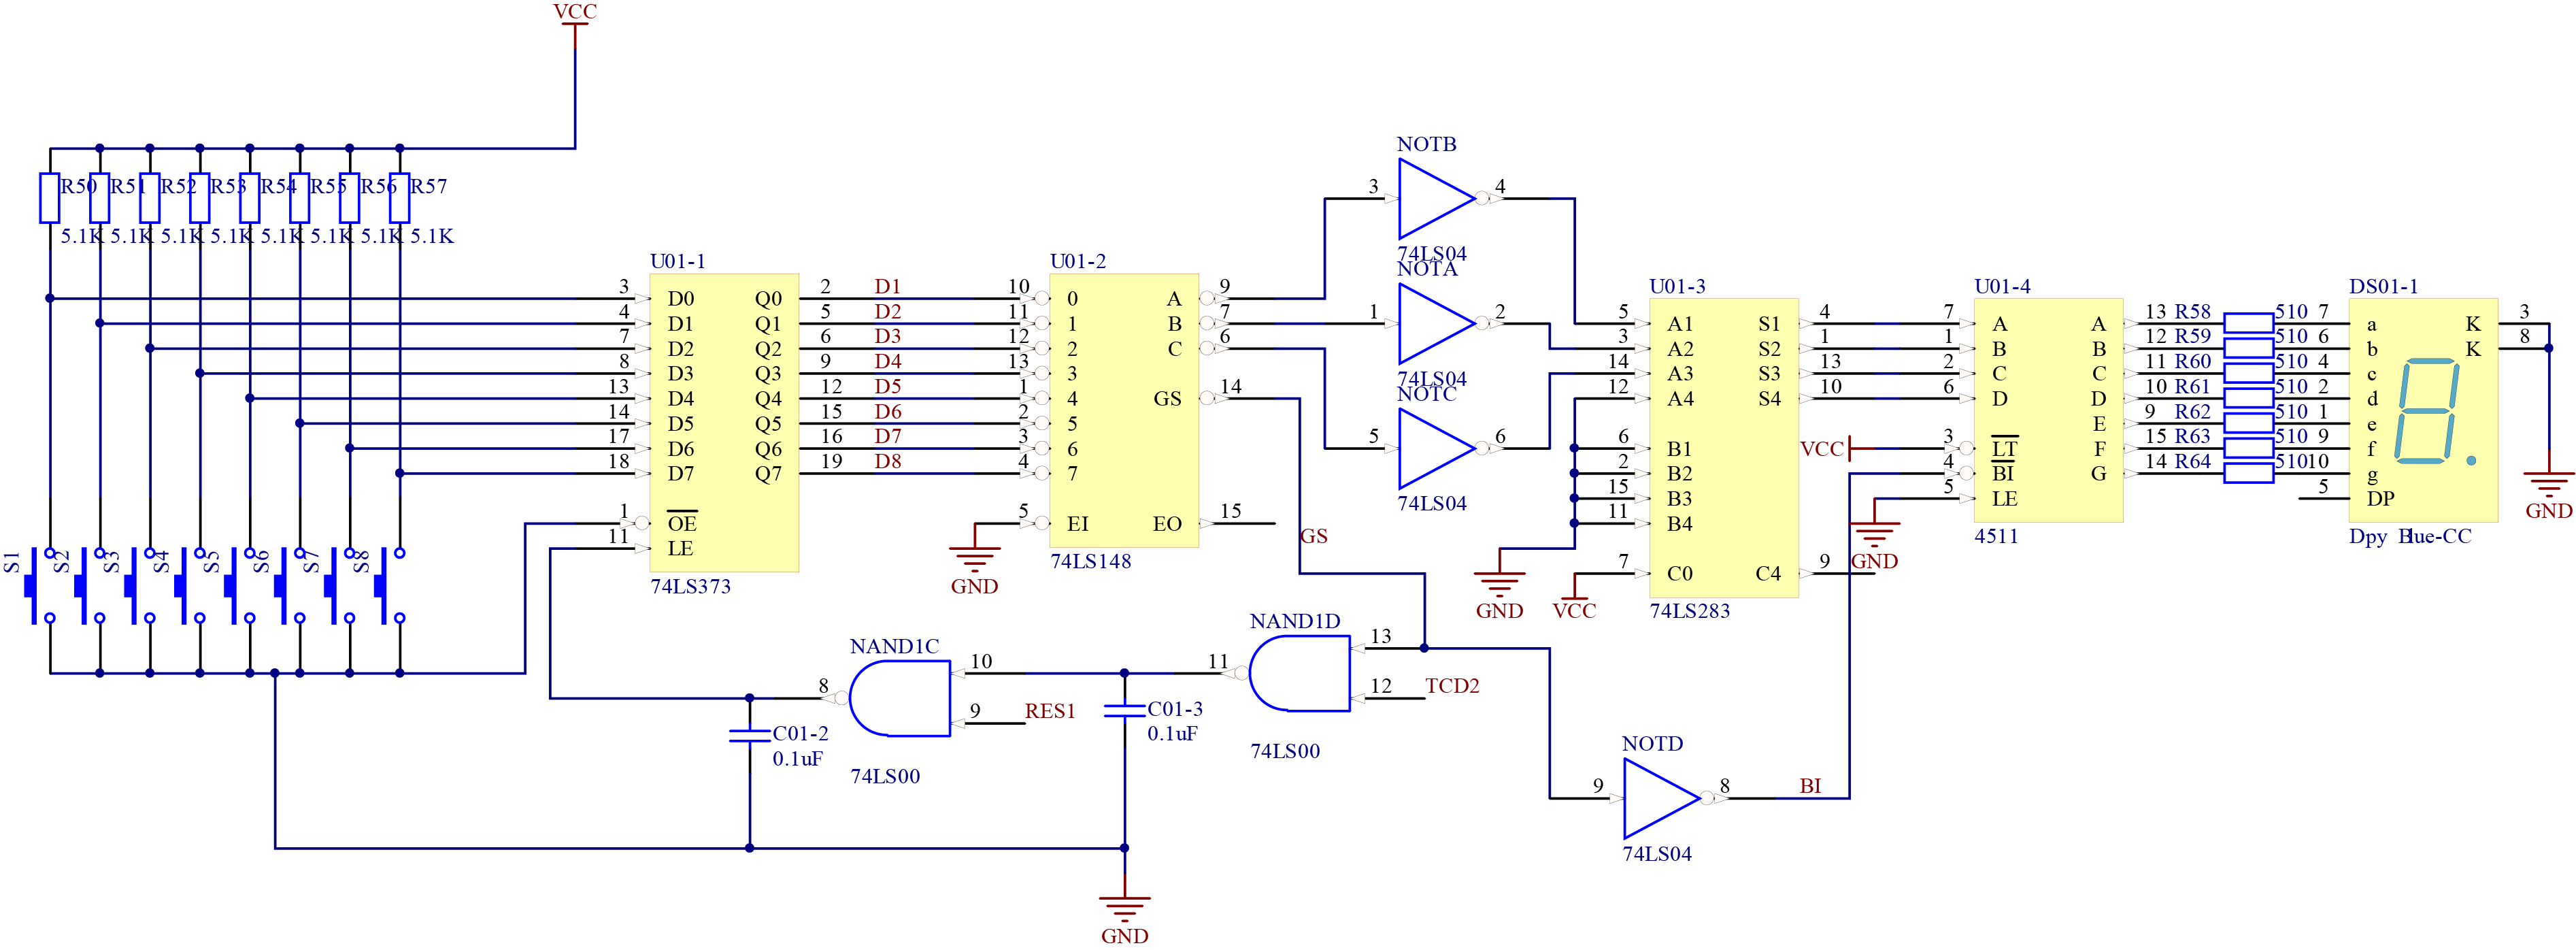
\includegraphics[width = 1\textwidth]{pic/P01.png}
                \caption{抢答输入、锁存、显示电路}
            \end{figure}
            电路组成:按钮开关S1~S8、数据锁存器74LS373、编码器74LS148、全加器74LS283、译码器CD4511、门电路及数码管等。

            主持人的复位开关产生一个负脉冲,使与非门G1输出高电平,加到锁存器74LS373的锁存控制端LE,使锁存器输出不锁定,并与输入端一致。此时S1~S8没有被按下,锁存器的输入端均为高电平,并反映到输出端,致使编码器74LS148的级联输出端GS为高电平,经与非门G2反相后得到低电平,使G1保持高电平输出,完成复位过程。

            抢答开始后,当某个输入按钮开关Si被按下时,对应的Di端为低电平,Qi端也为低电平,编码器GS信号立即转变为低电平,使门G1输出低电平,锁存器锁存控制端LE为低电平,执行锁存功能。这时若再有输入按钮被按下,锁存器的输出也不会发生变化,确保不会出现二次按键时的输入,起到封锁输入的目的。

            编码器的编码输出为反码,需经反相器反相后得到3位二进制码,由于参赛选手的编号为1~8,因此将编码器输出的编码通过全加器74LS283进行加1修正。修正后的数据送入BCD-七段译码器CD4511进行七段译码,由七段共阴数码管显示抢答者的组号。

            编码器级联信号GS反相后接译码器的灭灯信号BI的输入端,这样,在抢答成功前显示器不显示。编码器输出的这个信号还可作为抢答成功提示音的启动信号和倒计时停止计时的信号等。

        \subsection{可预置时间的倒计时定时器设计}
            \begin{figure}[H]
                \centering
                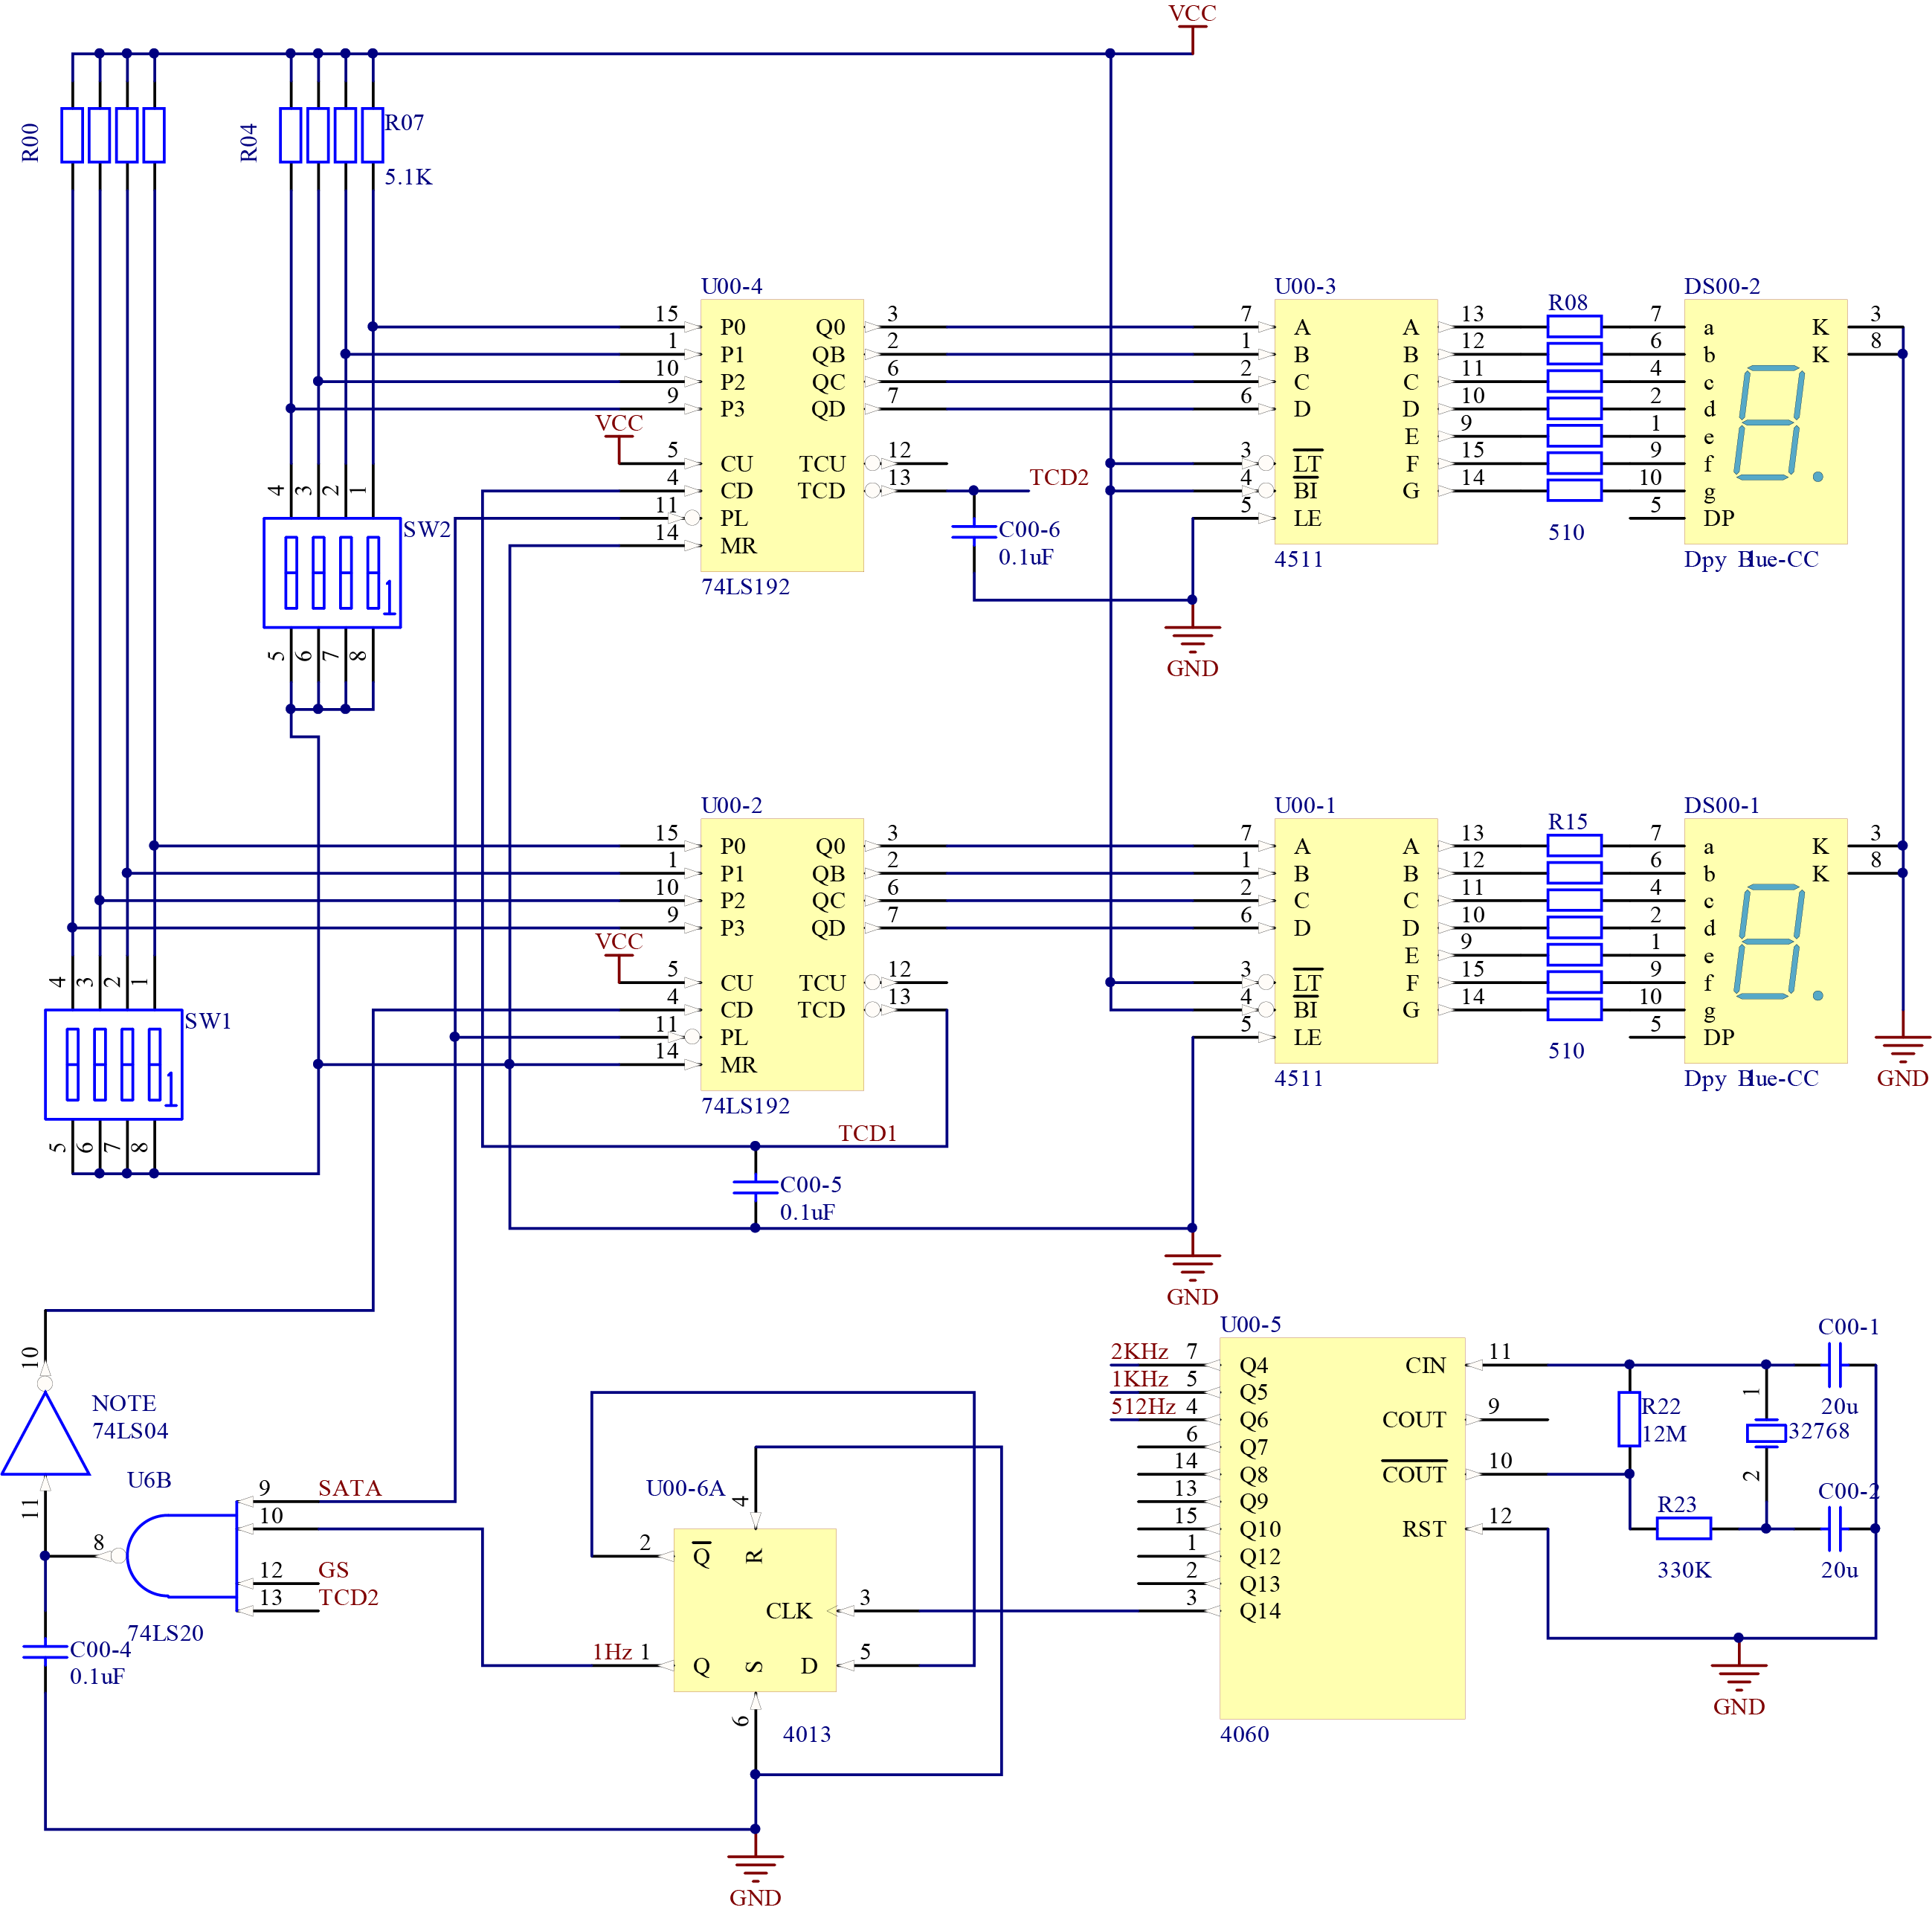
\includegraphics[width = 1\textwidth]{pic/P00.png}
                \caption{可预置时间的倒计时定时器设计}
            \end{figure}
            在抢答环节中,有时需要规定抢答的时间,如果超过规定的时间没有选手抢答,则停止本轮抢答。主持人可根据题目的难易程度在99秒范围内设定时间长短。

            电路组成:时钟专用电路4060、可预置数可逆计数器74LS192、译码器CD4511和共阴数码管等。
            
            由32768晶振电路产生32768Hz的信号,经过4060分频后得到2Hz~2KHz的信号,其中2Hz信号用于产生秒标准信号,其它输出信号可作为告警电路不同音效的音频信号。
            
            由CD4013主从D触发器组成的二分频信号将2Hz的信号转换为1H的秒标准信号经组合控制电路后作为计数器的计数信号。

            控制电路由一个与非门和一个反相器组成一个与门,实现计数器的启动由主持人的开始信号SATA启动,当主持人复位,或者抢答成功,或者倒计时结束时都要停止计数的功能。

            74LS192是一片可预置数的可逆计数器,在这里作减计数,每秒减1,低位计数减到О时,低位74LS192的借位信号TCD输出借位脉冲TCD1作为高位计数器的计数脉冲,从而实现高低位级联。当全部计数器都计到0时,高位计数器输出借位脉冲TCD2,此信号作为规定时间到信号,一方面封锁秒信号而停止计数,并启动提示音,另一方面封锁抢答输入电路,禁止选手再抢答。预置数由拨码开关设置,通过主持人的复位信号置入预置数。

        \subsection{抢答指示灯设计} 
            \begin{figure}[H]
                \centering
                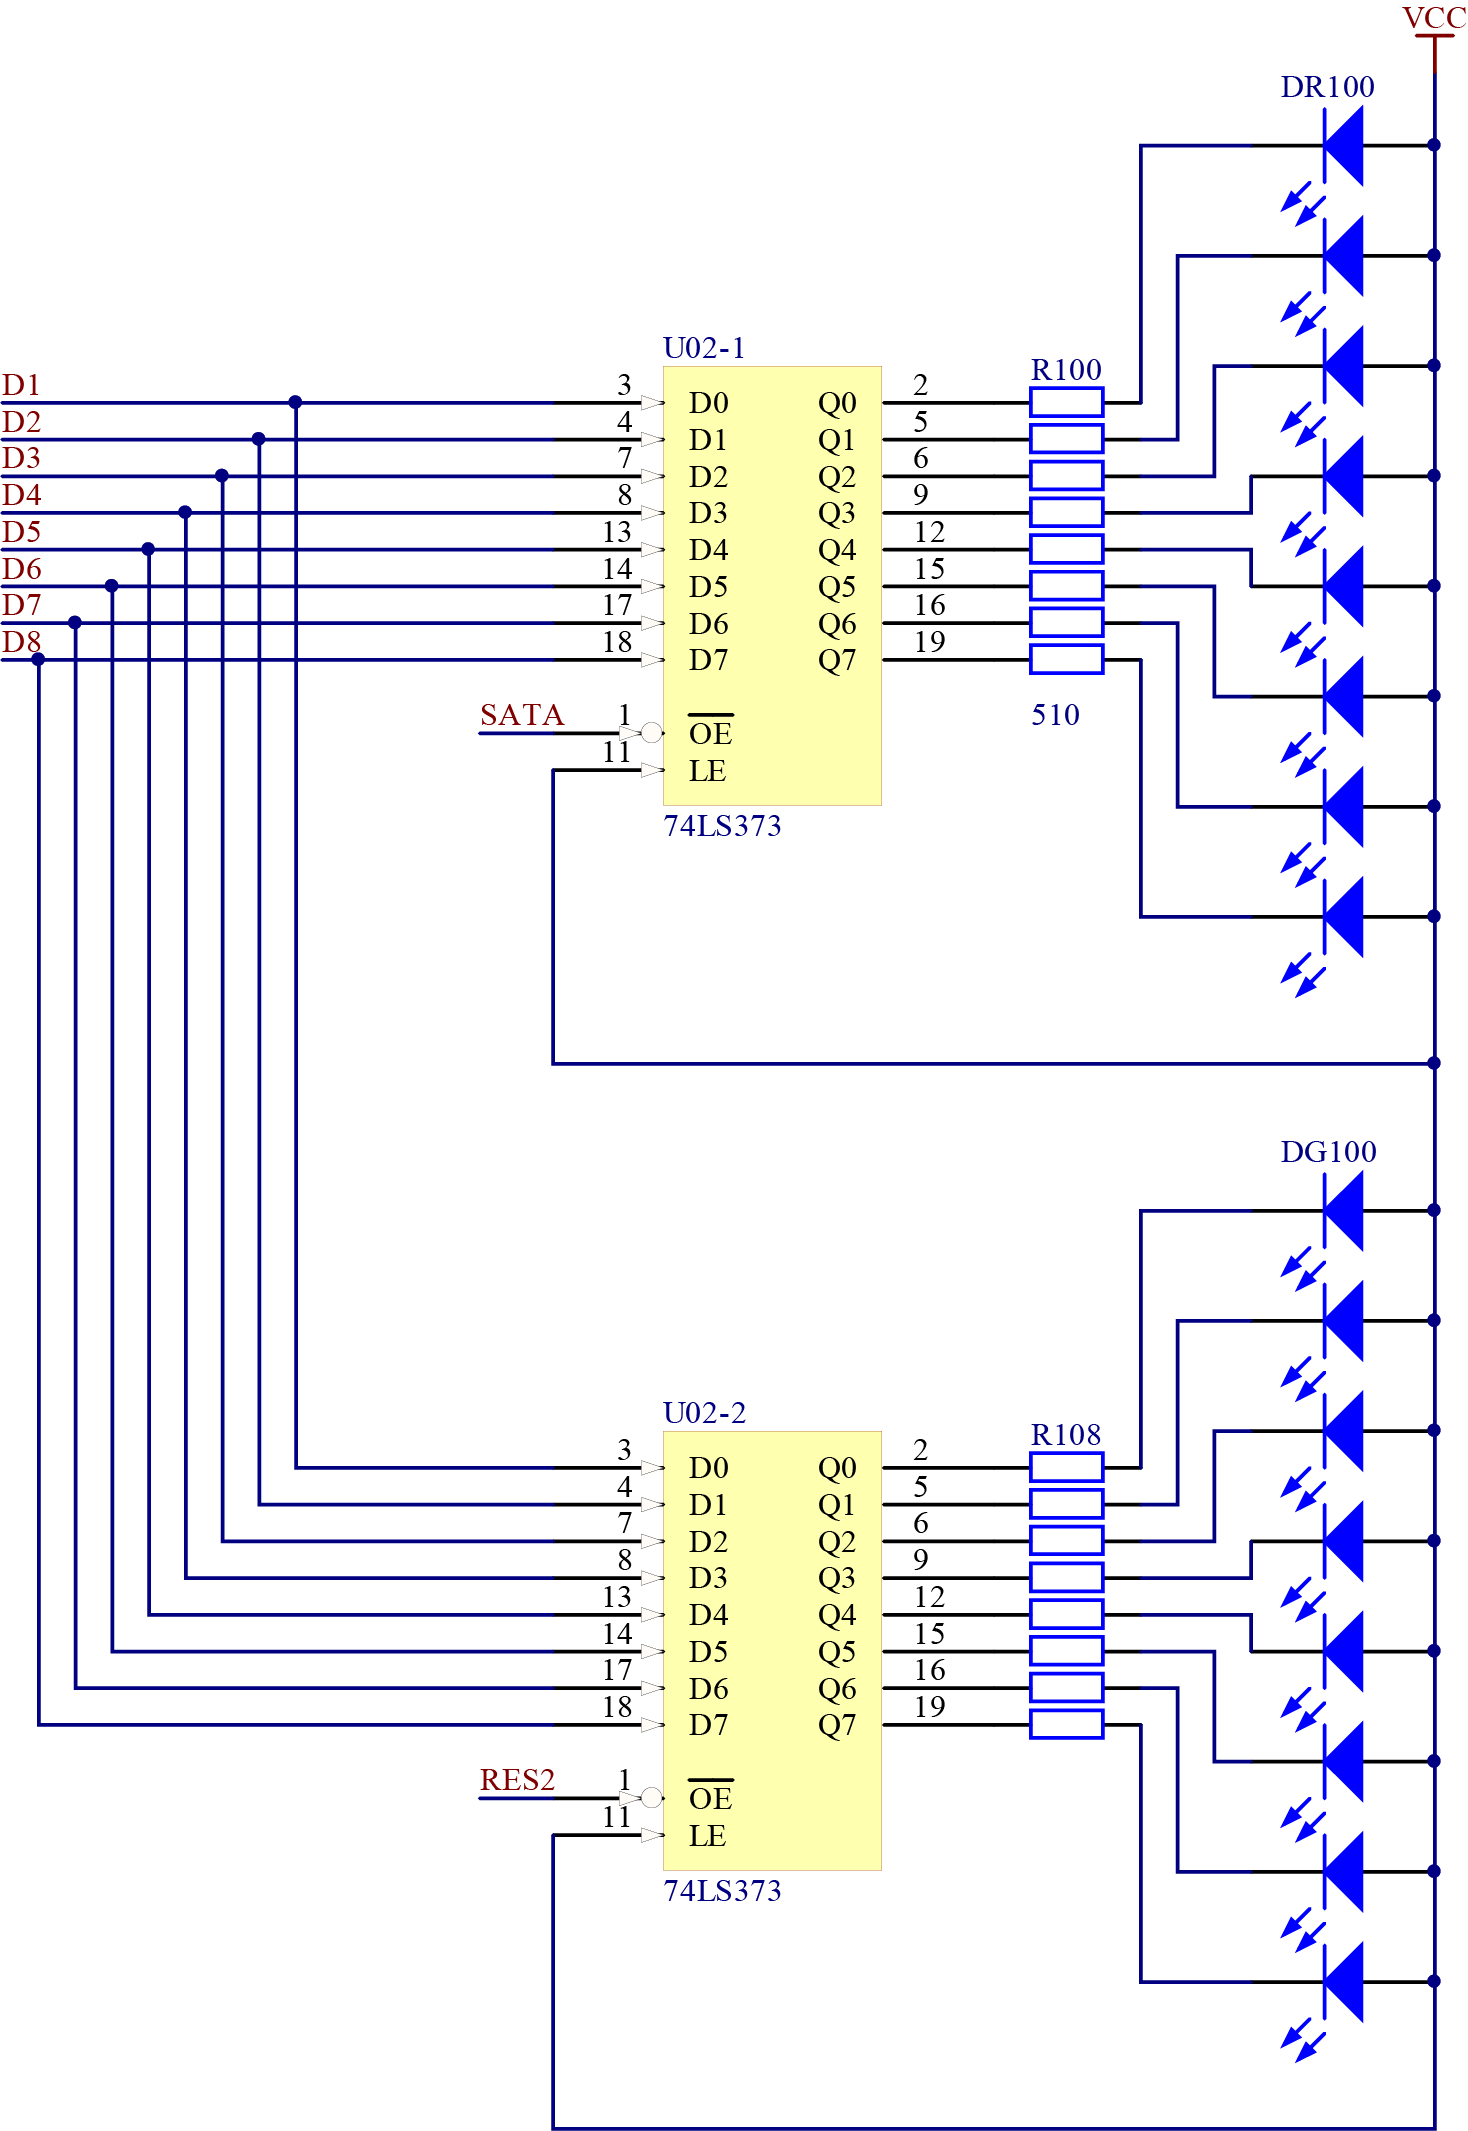
\includegraphics[width = 0.6\textwidth]{pic/P02.png}
                \caption{抢答指示灯设计}
            \end{figure}
            电路组成:发光二极管、74LS373锁存器等。

            为了给选手更直观地显示抢答成功与否,除了显示出组号外,在抢答器终端处设置指示灯,直观地指示出抢答成功者。指示灯设红、绿两个,绿灯表示抢答成功,红灯表示该选手提前抢答,属违规行为。抢答信号从锁存器的输出端获得,再结合主持人的开始信号判断出是抢答成功还是提前抢答。电路组成如图4所示。由主持人复位、开始信号分别控制锁存器的输出控制端,实现提前抢答或抢答成功的指示。

        \subsection{告警电路设计}
            \begin{figure}[H]
                \centering
                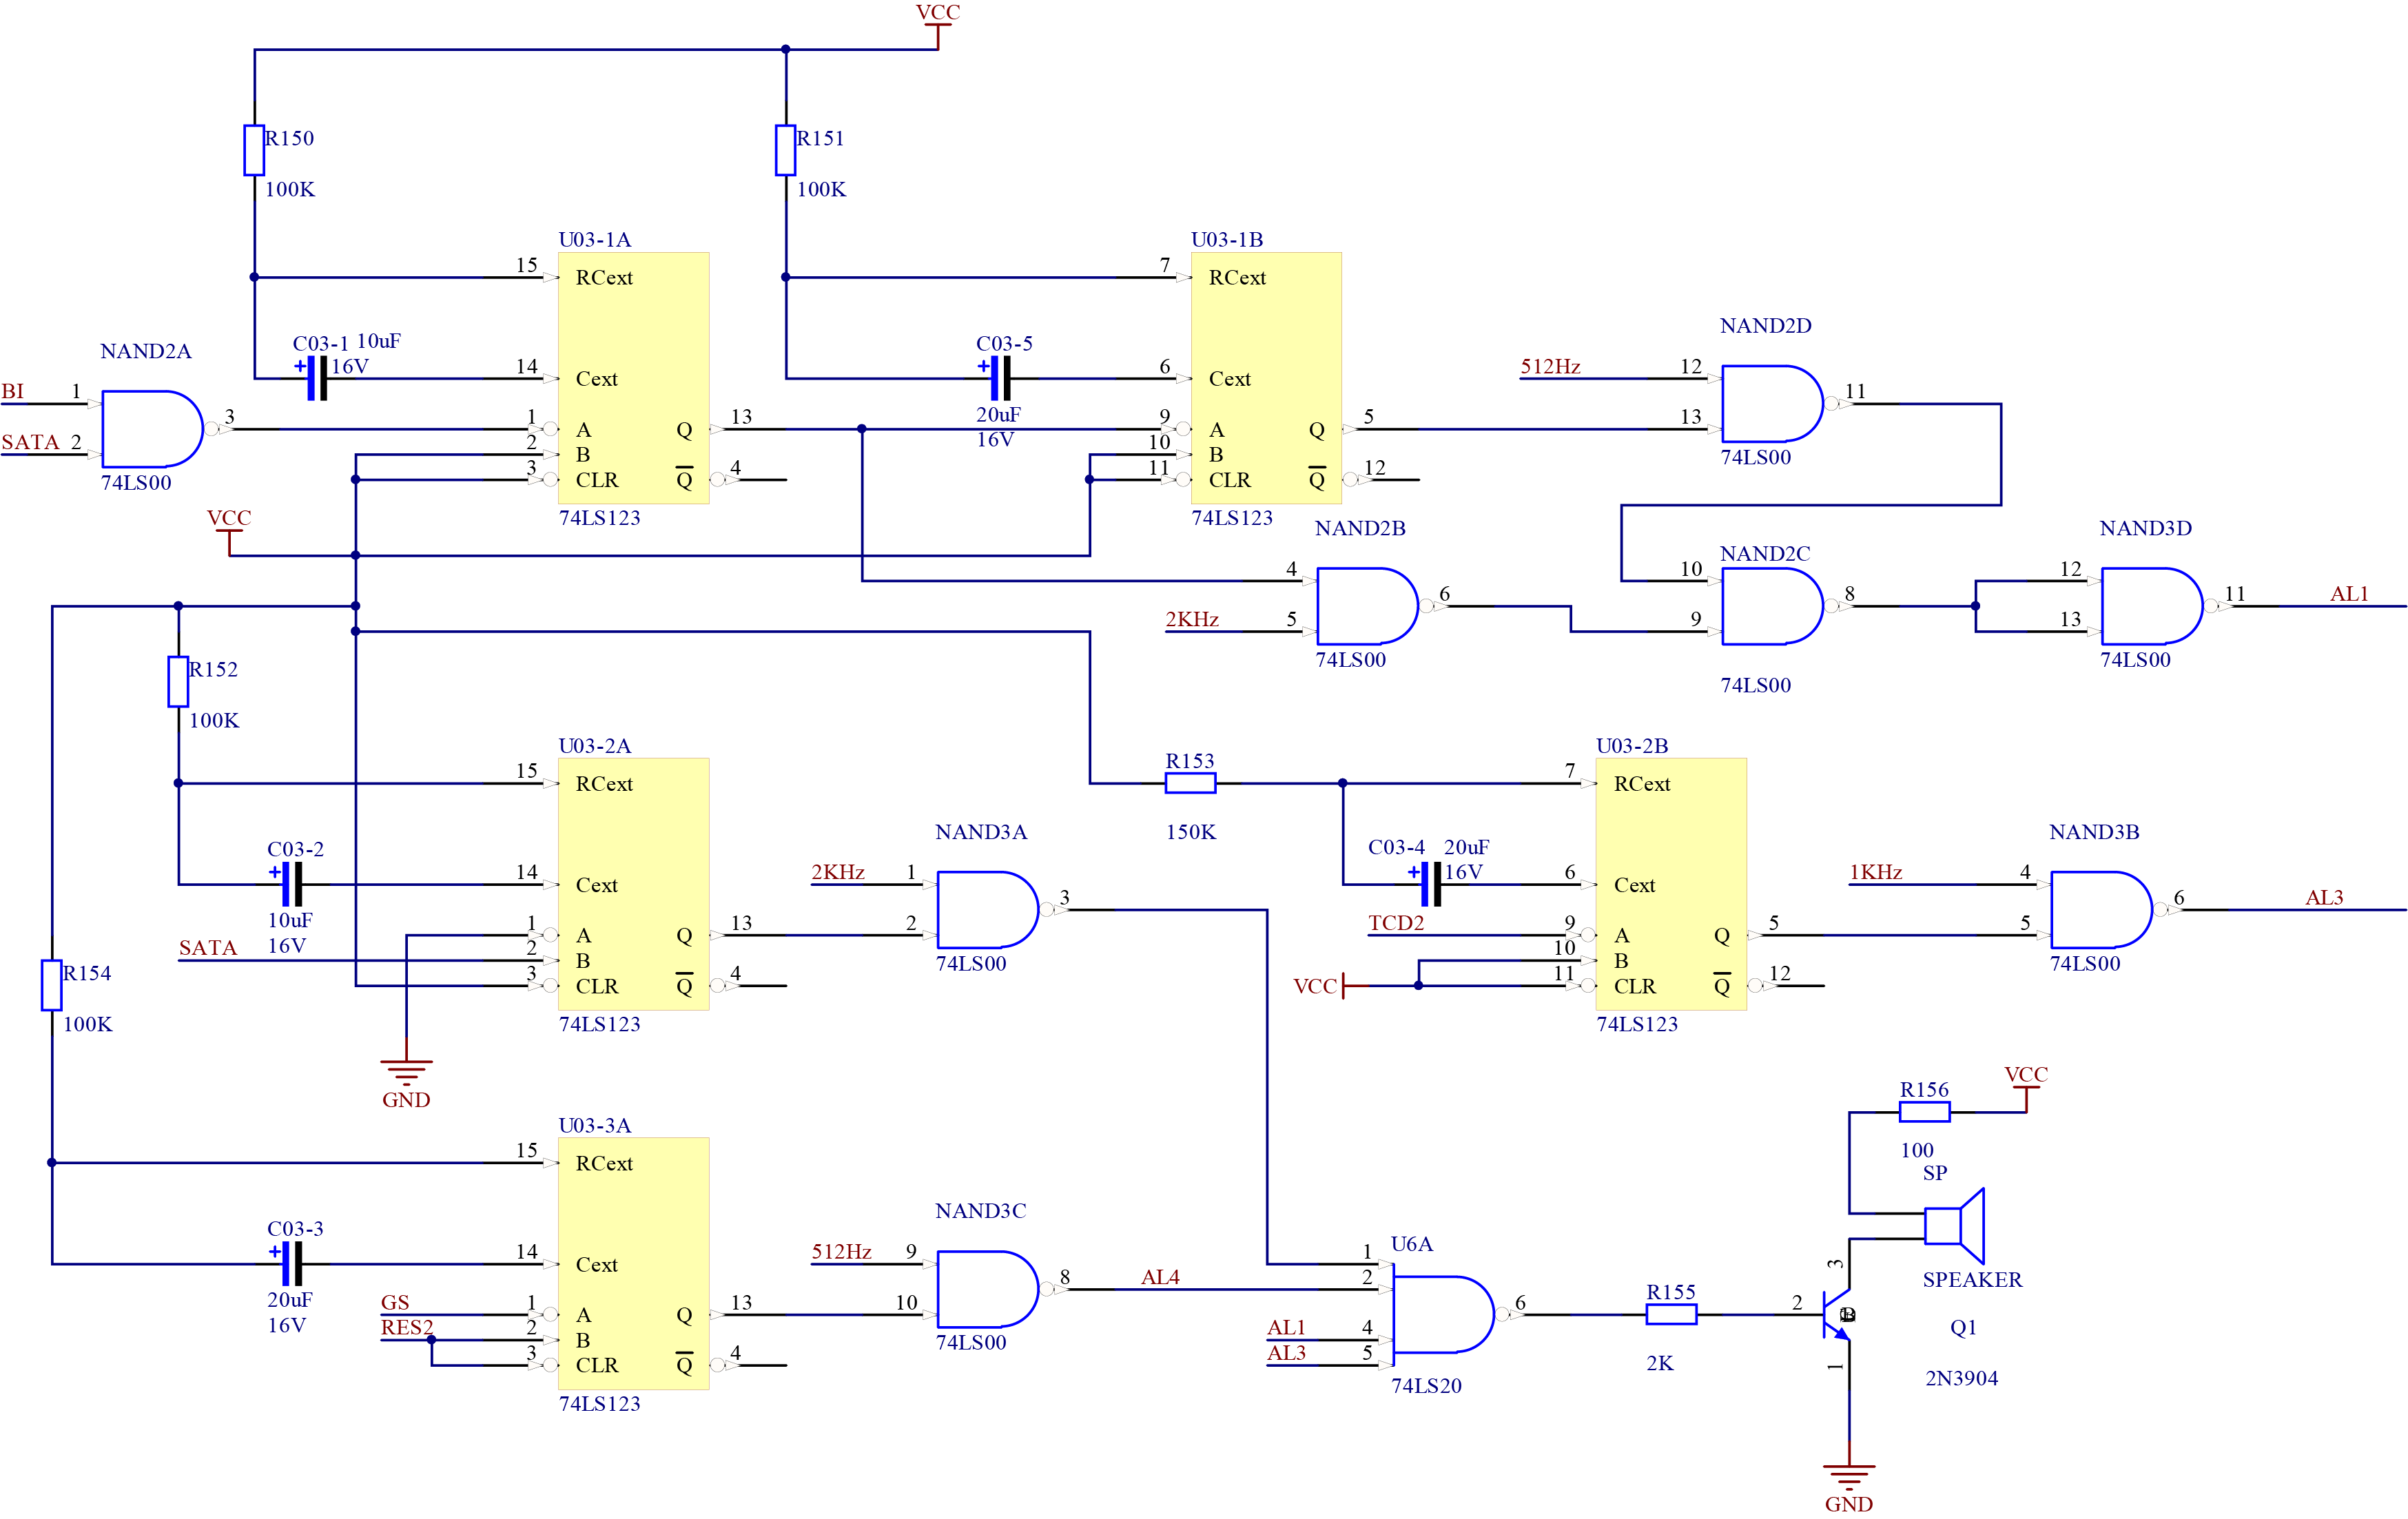
\includegraphics[width = 1\textwidth]{pic/P03.png}
                \caption{告警电路设计}
            \end{figure}

        告警电路的作用是当不同的操作发生时,给出相应的提示音,共有4种不同的提示音:
        \begin{enumerate}
            \item 抢答开始提示音:短促的“嘀”
            \item 抢答成功提示音:“嘀-嘟”
            \item 时间到提示音:长“嘟”音
            \item 提前抢答提示短暂“嘟”音
        \end{enumerate}
        
        电路组成:单稳态触发器74LS123、与非门等。

        用时钟电路的输出 (Q5=2048Hz、Q6=1024Hz、Q7=512Hz)作音频信号,用单稳态触发器74LS123控制音响时长,电路如图5所示。

        以抢答成功的“嘀-嘟”为例进行分析:

        当开始抢答并有人抢答成功时,BI从低电平变为高电平,SATA保持为高电平,两者相连的与非门产生一个下降沿信号,控制74LS123单稳态电路U03-1A产生一个$tw1 = 0.37\times 100K \times 10 \mu F = 0.37s$的稳态信号Q1,Q1与2KHz的信号组合最终经扬声器发出音高为2kHZ,持续时间为0.37s的“嘀”音;同时Q1单稳态结束时的下降沿信号控制74LS123单稳态电路U03-1B产生一个一个下降沿信号,控制74LS123单稳态电路U03-1A产生一个$tw2 = 0.37\times 100K \times 20 \mu F = 0.74s$的稳态信号Q2,在“滴”结束时Q2与512Hz的信号组合最终经扬声器发出音高为512HZ,持续时间为0.74s的“嘟”音。

        \subsection{控制电路设计}
        控制电路控制了整个抢答器的工作运行状态,是整个抢答器的关键,包括抢答输入封锁控制电路、倒计时控制电路、主持人控制电路等。
            \subsubsection{抢答输入封锁电路}
                \begin{figure}[H]
                    \centering
                    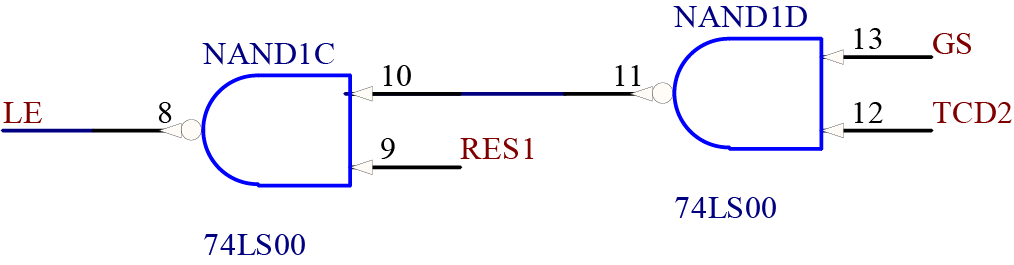
\includegraphics[width = 0.6\textwidth]{pic/封锁.png}
                    \caption{抢答输入封锁电路}
                \end{figure}
            抢答封锁控制受倒计时结束输出TCD2、抢答编码器级联输出GS和主持人的控制。当倒计时计数结束时TCD2为低电平,这时编码器无输入,GS 为高电平;而当有选手抢答时,编码器GS输出低电平,这时TCD2为高电平;当主持人手动复位时,解除封锁并返回到初始状态。
            \subsubsection{倒计时控制电路}
                \begin{figure}[H]
                    \centering
                    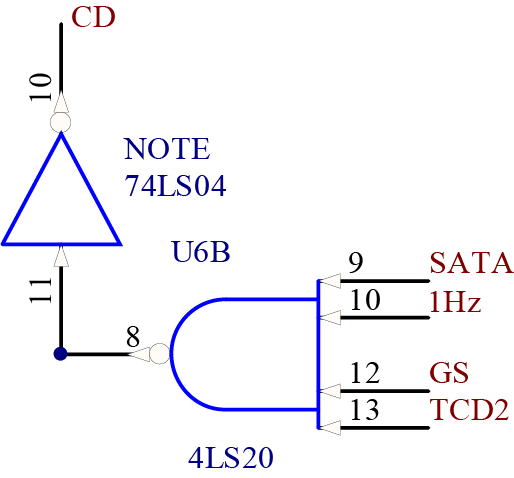
\includegraphics[width = 0.3\textwidth]{pic/倒计时.png}
                    \caption{倒计时控制电路}
                \end{figure}
            倒计时也受TCD2、GS 控制和主持人控制,当TCD2和GS中任何一个信号为低电平时,封锁秒信号而停止计数,当主持人手动开始时启动计数,当主持人复位时计数器置入预置数。
            \subsubsection{主持人控制电路}
                \begin{figure}[H]
                    \centering
                    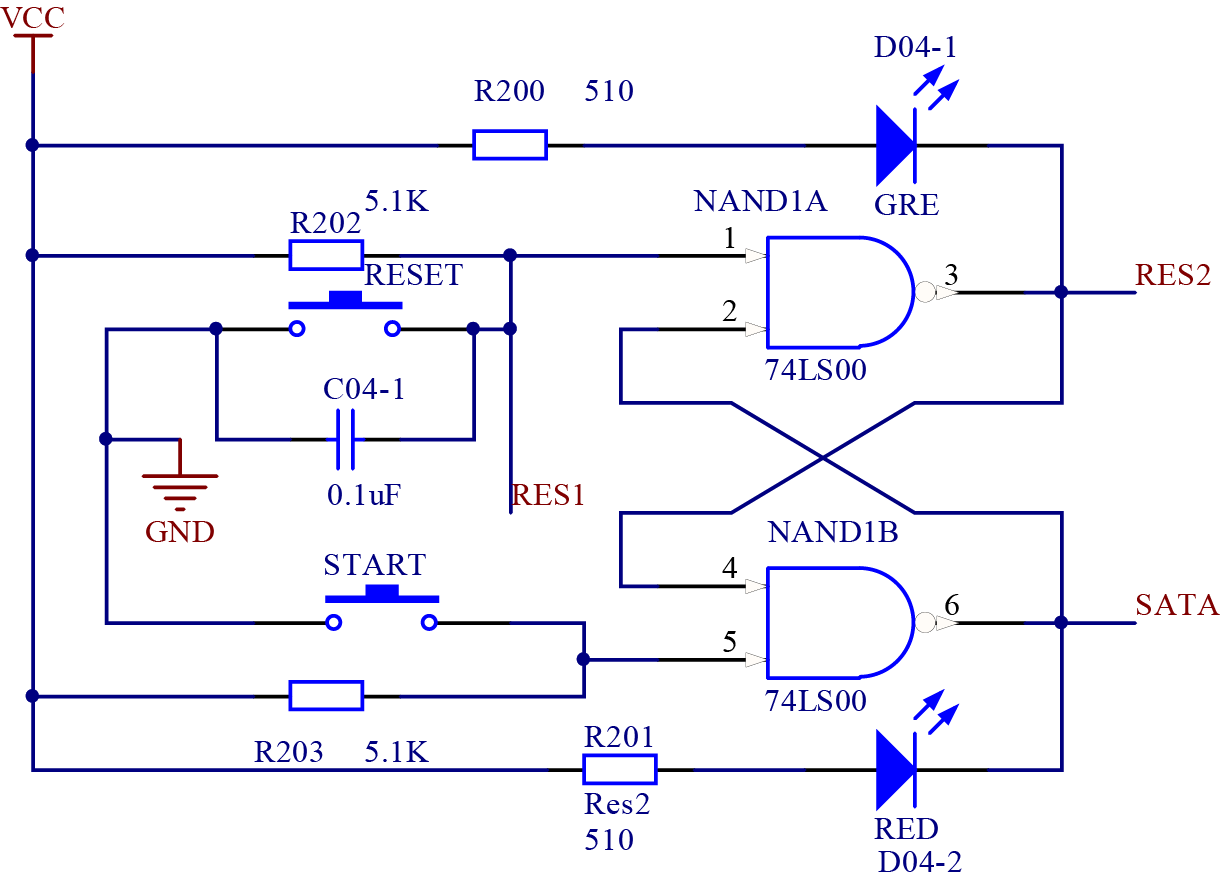
\includegraphics[width = 0.7\textwidth]{pic/P04.png}
                    \caption{主持人控制电路}
                \end{figure}
            机械开关在拨动时会有抖动现象,这些抖动会严重影响电路的工作,必须设法将它去除。主持人控制电路实际上仅仅控制了系统的“复位”和“开始”,用基本R-S触发器去除抖动,用一个滤波电容去除RES1信号的抖动。
            
            当主持人按下复位按钮(RES)后,产生一个下降沿信号RES1,同时RES2由低电平转换为高电平并保持,SATA由高电平转换为低电平并保持,红灯亮;当主持人按下开始按钮(SAT)后,SATA由低电平转换为高电平并保持,RES2由高电平转换为低电平并保持,绿灯亮。
        \subsection{计分电路设计}
            \begin{figure}[H]
                \centering
                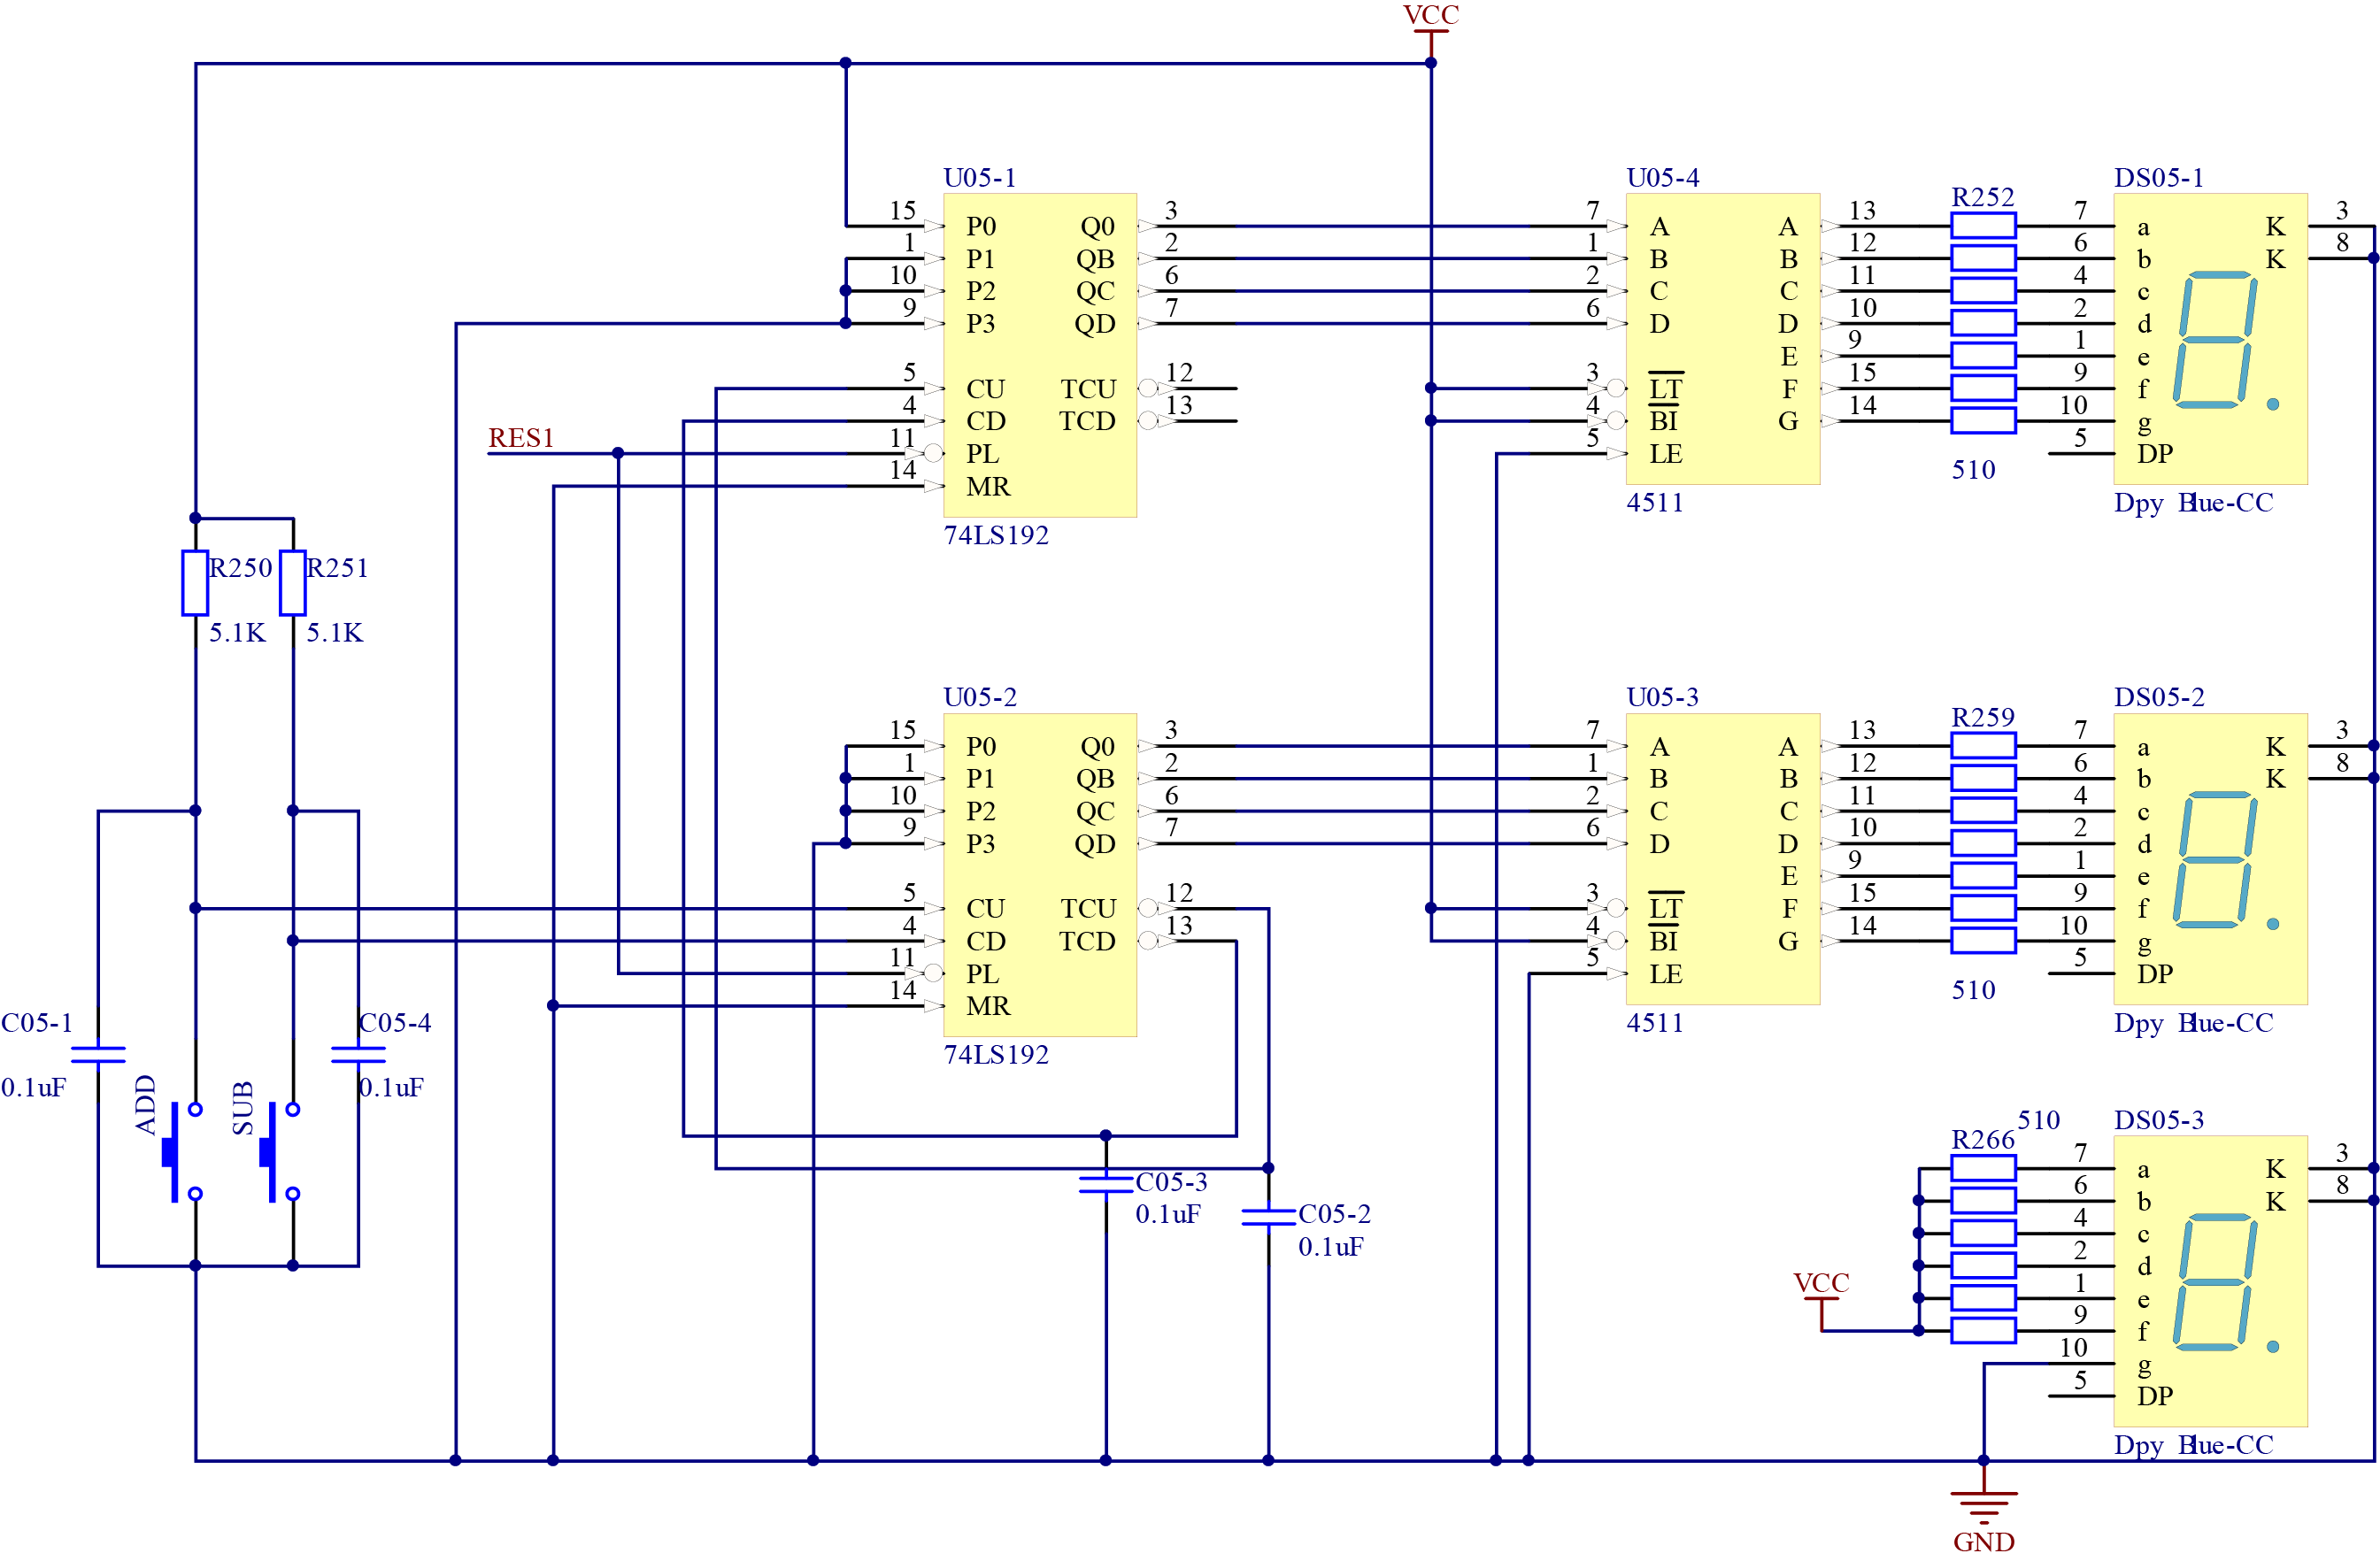
\includegraphics[width = 1\textwidth]{pic/P05.png}
                \caption{计分电路设计}
            \end{figure}
        电路组成:按钮ADD,SUB、74LS192可逆计数器、CD4511译码器和共阴数码管等。

        计分电路由3个数码管组成,由于每次都是加(减〉10分,个位数始终为0,所以只要对十位和百位进行加(减)计数即可,个位仅用数码管显示0。

        主持人复位时,RES1信号控制两个74LS192可逆计数器置入预置数进行复位,数码管复位为100 。

        计分时,主持人可以通过加分按钮ADD、减分按钮SUB进行加减分控制。两个按钮产生的信号分别控制74LS192可逆计数的加计数和减计数,实现计分。


        \subsection{开关按钮消抖设计}
        设计时我们采用并联一颗0.1uF的陶瓷电容,进行滤波处理来消除开关的抖动(调试时发现这样的设计并不能达到消抖的目的,在后文我们进行了新的设计)。
        \subsection{竞争-冒险消除}
        在分析可能产生竞争-冒险现象的元件出,我们采用在输出端接入滤波电容来消除竞争冒险现象。
        \subsection{电源模块设计}
                \begin{figure}[H]
                    \centering
                    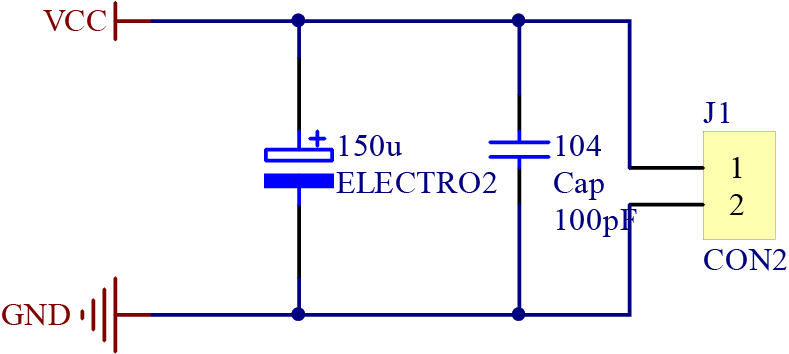
\includegraphics[width = 0.5\textwidth]{pic/source.png}
                    \caption{电源模块设计}
                \end{figure}
            电源输入5V电压,同时并联一个150uF的极性电容进行滤波,一个0.1uF的小电容滤除高频。
        \subsection{关键信号的获得与作用}
            \begin{enumerate}
                \item 主持人复位信号RES1:主持人按下复位按钮后产生一个下降沿脉冲,主要用于倒计时抢答封锁电路的复位。
                \item 主持人复位信号RES2:主持人按下复位按钮后,通过RS触发器获得一个高电平的信号RES2,重要用于控制一些电路的复位。
                \item 主持人开始信号SATA:主持人按下复位按钮后,通过RS触发器获得一个高电平的信号SATA,重要用于控制抢答的开始和一些复位(由于SATA与RES2作为了RS触发器的两个输出端,所以SATA可以作为RES2的反相输出)。
            \end{enumerate}
        \subsection{元器件清单}
            \begin{table}[H]
                \centering
                \caption{元器件清单}
                \begin{tabular}{|c|c|c|c|}
                    \hline
                    型号          & 功能             & 数量 & 封装          \\ \hline
                    4013        & 双主-从D型触发器      & 1  & DIP-14      \\ \hline
                    4060        & 14级二进制串行计数/分频器 & 1  & DIP-16      \\ \hline
                    4511        & BCD锁存7段译码驱动器   & 5  & DIP-16      \\ \hline
                    74LS00      & 2输入端四与非门       & 3  & DIP-14      \\ \hline
                    74LS04      & 六反相器           & 1  & DIP-14      \\ \hline
                    74LS20      & 4输入端双与非门       & 1  & DIP-14      \\ \hline
                    74LS123     & 双可再触发单稳态多谐振荡器  & 3  & DIP-16      \\ \hline
                    74LS148     & 8 线-3 线优先编码器   & 1  & DIP-16      \\ \hline
                    74LS192     & 可预置BCD双时钟可逆计数器 & 4  & DIP-16      \\ \hline
                    74LS283     & LED+F11:K11    & 1  & DIP-16      \\ \hline
                    74LS373     & 三态同相八D锁存器      & 3  & DIP-20      \\ \hline
                    SW-PB       & 小按键            & 12 & AN-S        \\ \hline
                    Dpy Blue-CC & 7段数码管          & 6  & H           \\ \hline
                    LED         & 绿色LED          & 9  & LED-3       \\ \hline
                    LED         & 红色LED          & 9  & LED-3       \\ \hline
                    XTAL        & 石英晶体振荡器        & 1  & XTAL1       \\ \hline
                    SPEAKER     & 喇叭             & 1  & RAD-0.2     \\ \hline
                    SW DIP-4    & 四位拨码开关         & 2  & DIP-8       \\ \hline
                    CON2        & 2线电源插座         & 1  & POWER PLUG2 \\ \hline
                \end{tabular}
            \end{table}
    \section{PCB板图设计}
            \begin{figure}[H]
                \centering
                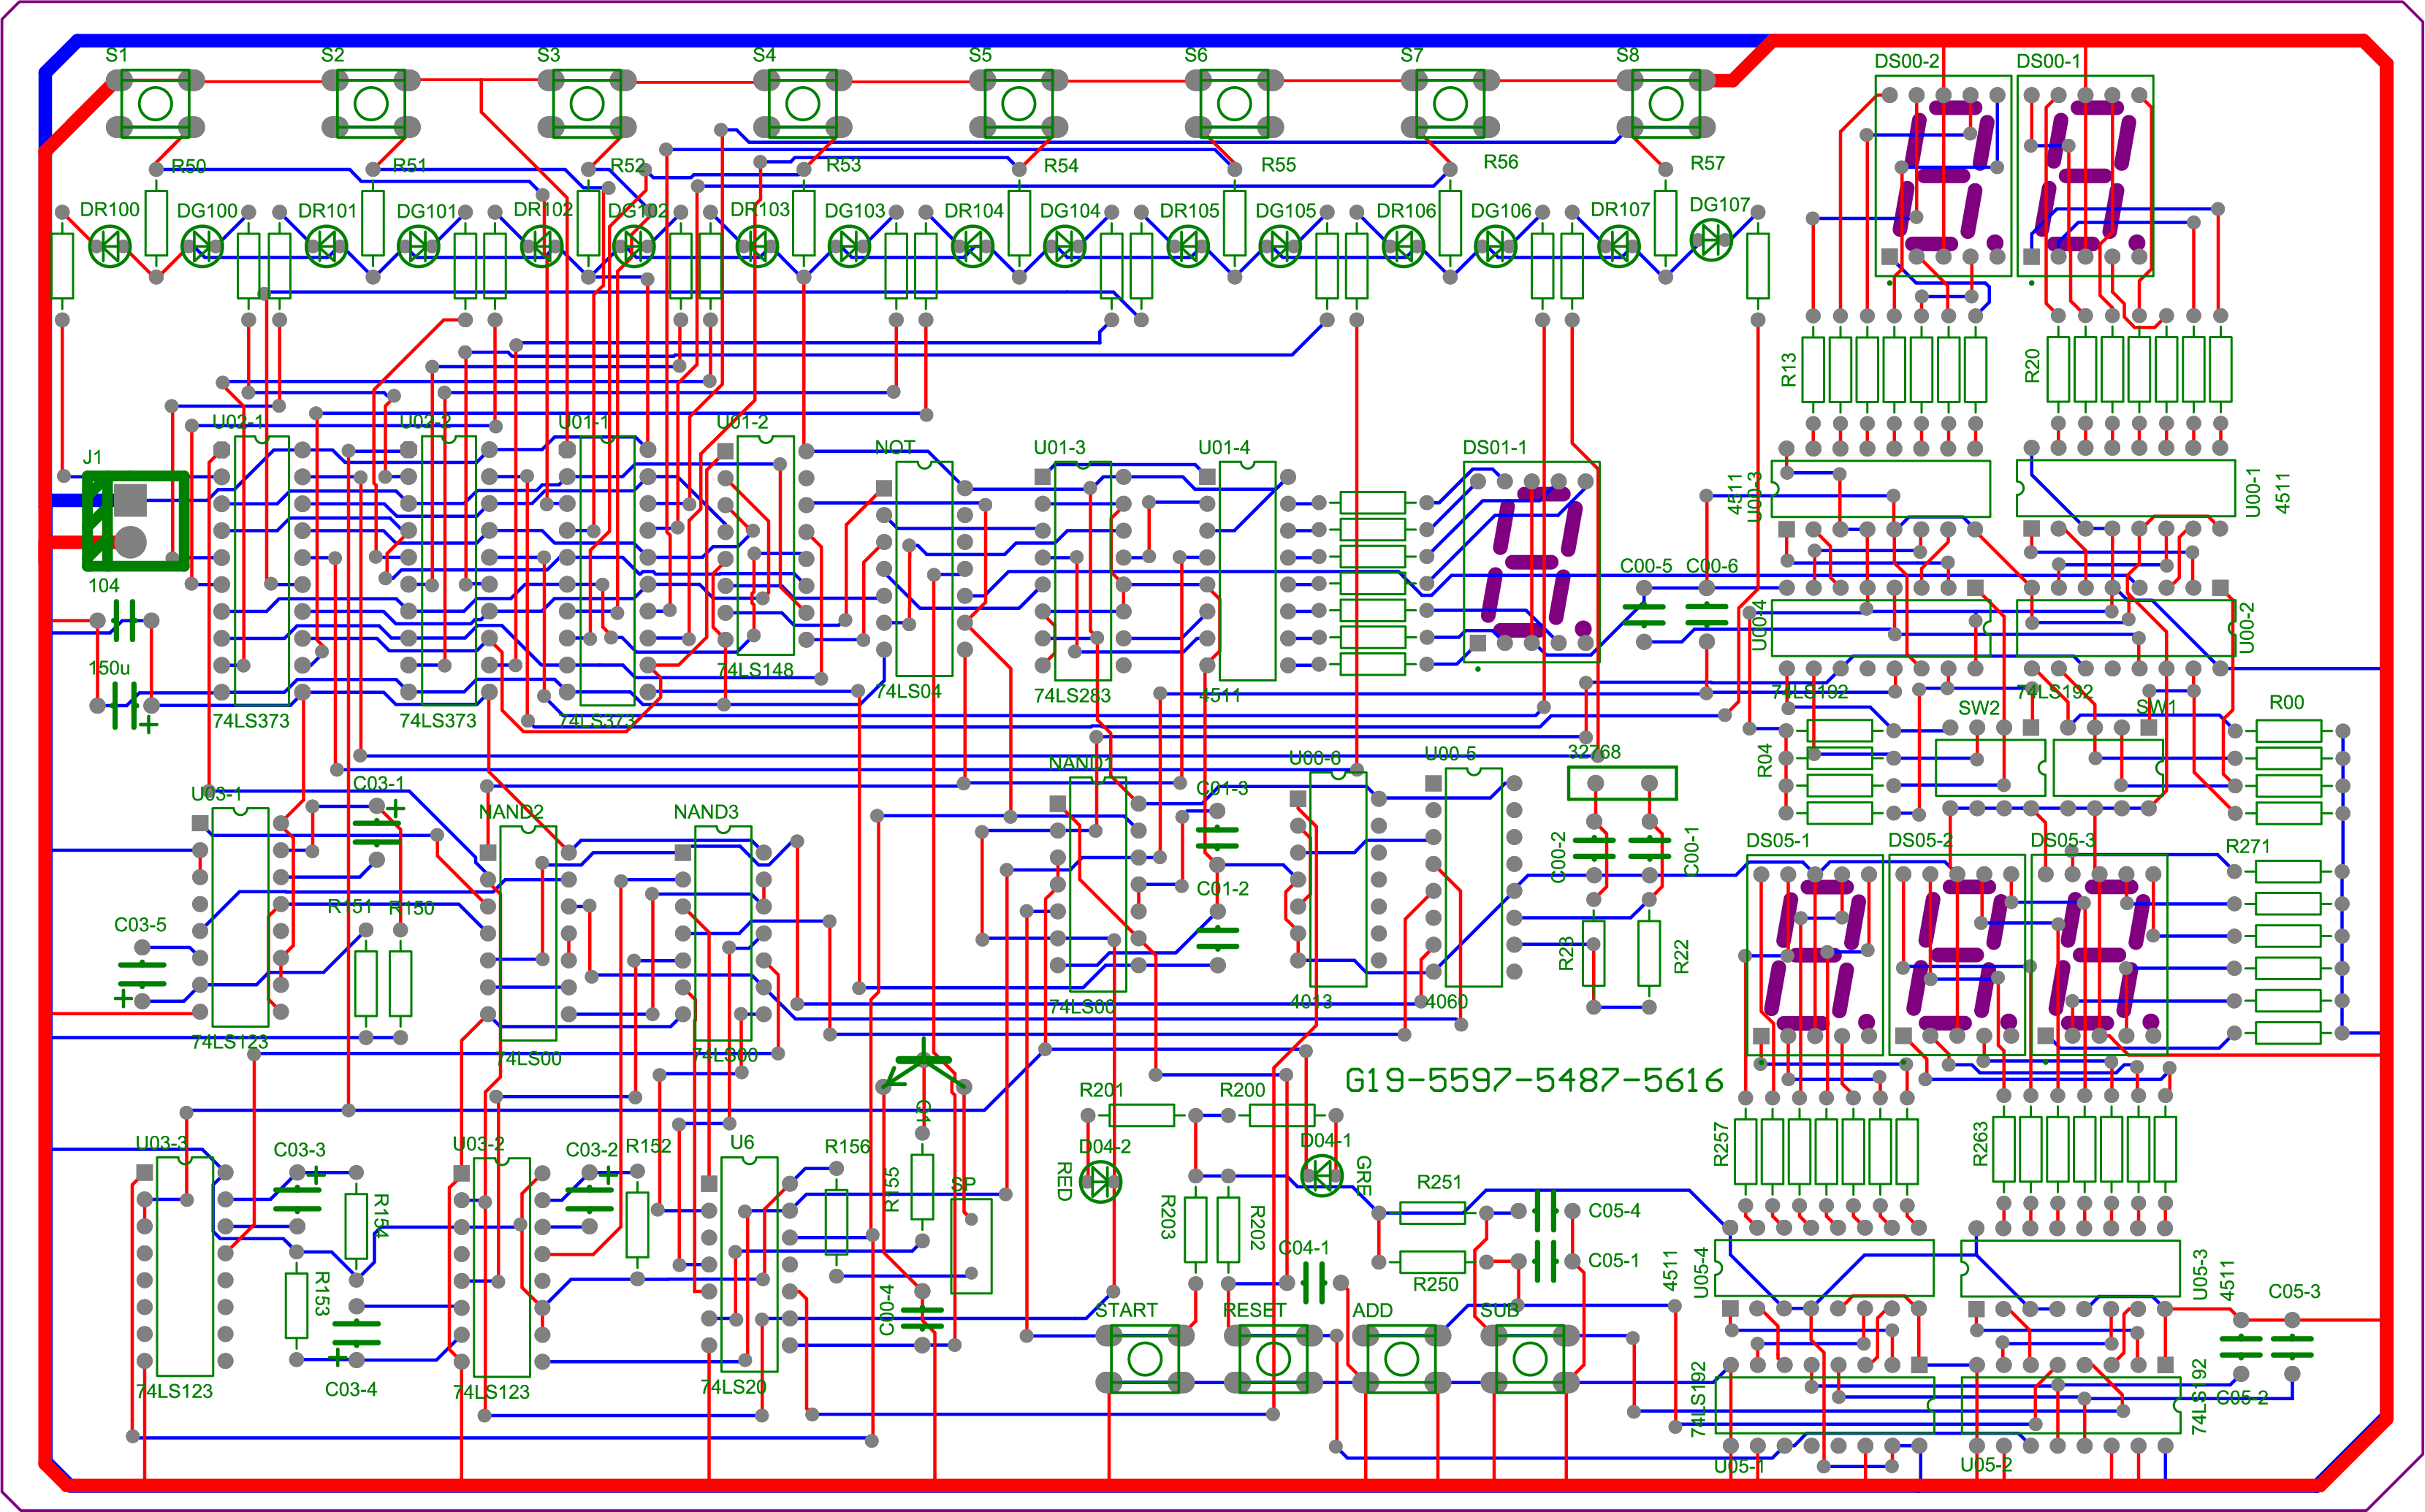
\includegraphics[width = 1\textwidth]{pic/pcb.png}
                \caption{PCB图}
            \end{figure}
            在进行元器件吗的布局时,我们按照电路的功能,将电路分成了7个不同的模块,并且按照模块将元器件放在一起,同时根据元器件之间的连线对模块内的元器件进行了合理的布局与排布,尽量降低连线时的复杂程度。

            连线时,由于电路比较复杂,所以我们采用了打过孔的方法,顶层的红线尽量竖直,底层的蓝线尽量水平,而两种线通过过孔进行交接,同时我们稍微增大了连线较为复杂的元器件之间的距离,这样极大的提高了线路连接的速度与效率。

    \section{安装与调试}
        \subsection{电路板焊接}
            拿到电路板后,我们按照从低到高的原则对元器件进行了焊接。
            \begin{figure}[H]
                \centering
                \includegraphics[width = 1\textwidth]{pic/实物图.jpg}
                \caption{多路竞赛抢答器}
            \end{figure}
        \subsection{电路调试}
            完成焊接上电后,我们发现了一些问题,并调试解决。
            \subsubsection{抢答成功的提示音只有“嘟”,并不是“嘀嘟”。}
            我们最开始怀疑是控制“嘀”时长的74LS123单稳态芯片出了问题,所以我们将另外一个74LS123单稳态芯片与之互换,结果问题还是存在,便排除了芯片的问题。

            我们又用万用表测试了“嘀”的74LS123单稳态芯片的输出电压,发现在本应该是“嘀”音时为高电压44的输出端检测到的电压只有0.65V左右。

            之后我们仔细分析了问题的成因,由于“嘟”音是通过“嘀”的74LS123单稳态芯片产生的单稳态波形的下降沿触发的,而“嘟”音有,则说明“嘀”的74LS123单稳态芯片是产生了单稳态波形。但是并没有听到“嘀”音,则说明“嘀”的74LS123单稳态芯片是成功产生了单稳态波形,只是由于单稳态的持续时间tw1太短,而未能产生“嘀”音,但是能触发“嘟”音的单稳态。

            这样问题就锁定在了是什么导致了“嘀”的74LS123单稳态芯片产生的稳态的持续时间tw1太短。我们在仔细检查了电路连接发现控制“嘀”的74LS123单稳态芯片tw1的电容大小出了问题。本应是10uF的电容,由于拿错元器件焊成了1uF的电容,从而导致了稳态的持续时间tw1太短。

            在更换了电容后问题得到了解决。
            \subsubsection{倒计时计数的时候是每2秒递减,并不是每一秒递减。}
            我们首先怀疑是4060产生的2Hz的信号出了问题,于是我们用示波器测了4060产生的2Hz信号,发现没有问题,于是我们继续用示波器测试二分频电路产生的1Hz秒信号,发现也无问题后我们开始分析电路原理的原因。在初步分析后我们怀疑是我们用以消除组合控制电路竞争冒险的0.1uF的滤波电容选取不合适,于是我们更换了20pF的电容,更换后问题得到解决。
            
            \subsubsection{计分电路开关抖动没有被消除。}
            在测试计分电路的时候,我们发现加减分按钮的抖动并没有被消除。我们初步认为是消除抖动的滤波电容的大小选取出了问题,在更换了电容后发现问题还是存在,在咨询了老师后,我们意识到是我们设计的利用电容滤波的消抖电路无效,但是PCB板已经打印出,如果此时去改电路的话是不现实的。所以我们放弃了这个模块的调试。

            虽然不能更改了,但是在查阅资料后,我们还是对此处的开关消抖电路进行了重新设计:
            \begin{figure}[H]
                \centering
                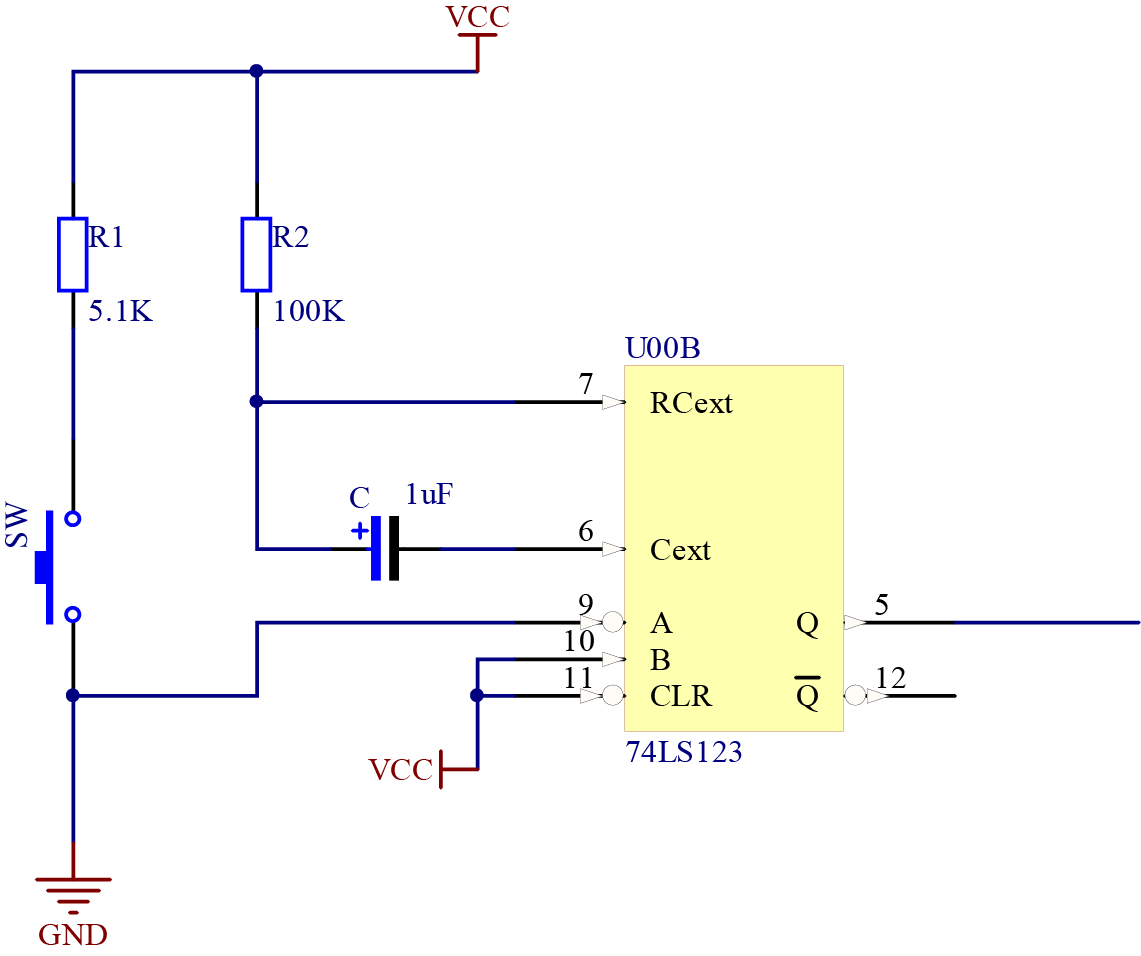
\includegraphics[width = 0.5\textwidth]{pic/消抖.png}
                \caption{改进后的消抖电路}
            \end{figure}
            我们采用了一个可再触发单稳态多谐振荡器电路对按钮的信号做了消抖处理如图。
            \subsubsection{设计调试方法总结}
            在原理图设计的时候应该多方面考虑,因为如果原理图设计不合理的话,会影响到后期的PCB板图设计与排线;同时,由于最后电路板打印好后很难再去修改电路,所以在设计原理图的时候也要尽量保证电路设计的合理。
            
            调试时可能会出现比较多的问题,这个时候应该将问题归类,按照一定顺序解决问题。同时调试的时候应该按照一定的顺序测试,比如首先检查元器件是否选错,排线是否正确;再检查电路设计是否合理,一步一步来。
    \section{心得与体会}
        在课程开始的时候,我们面对众多的选题迟迟无法确定选哪一个选题。于是我们小组成员一起查看每一个选题的文档介绍,仔细分析选题的难点和关键点。在初步查看完所有的选题后,我们选定了多路竞赛抢答器这个选题。

        在确定选题后我们开始了电路原理图的绘制。我们首先仔细分析阅读了文档介绍,由于老师所给的文档比较详实,所以我们很快就弄清了设计思路,并且分工进行了原理图的绘制。

        在绘制完成了基本的电路图后,在需要我们设计的地方我们小组成员一起对这些地方进行分析。
        
        首先我们对实验室没有的74LS集成芯片进行了替换,我们后来发现并不能直接简单地将74LS芯片替换为CD系列,有一个芯片替换的时候我们没有注意引脚区别,后来在检查电路的时候才发引脚接错了,原来的74LS芯片的LE引脚是低电平有效,但是更换为CD系列后这个引脚为高电平有效,但是我们在替换的时候就没有注意到这个问题,导致电路出错。万幸的是是在PCB布线前查出来的问题,仍然有修改的余地。这个问题也给我们提了一个醒,我们便仔细检查了我们所有的有过芯片替换的地方,确保替换芯片后没有问题。最后的确发现了问题,便是文档中用的译码器为74LS247是输出低电平有效,所以之后是驱动的共阳数码管,但是我们将译码器换成CD4511后,由于其输出是高电平有效,所以相应地要将数码管更换成共阴。

        二分频模块是杜秉哲提出可以用一个D触发器进行分频。倒计时组合控制模块的设计是由我们三人一起讨论,从分析功能到列出真值表再到最后确定元器件选择一步一步完成的。

        加分电路的设计也是在我们设计完成基本功能模块,在弄清了基本电路的功能原理后在我们讨论下设计出来的。

        在设计PCB板图时,我是主要负责设计PCB板图的组员。这个部分的设计让我深刻体会到合理布局的重要性,有时如果一个元器件位置布局不合理,往往会影响到周围很多元器件的布局,牵一发而动全身。
        
        同时PCB和成功设计和布局与原理图的设计有着密不可分的关系。在设计原理图时,我就将不同模块的原理图分开,并且元器件对元器件的命名进行了规范处理。这样在PCB排版的时候只有看到元器件的命名就可以直接知道这个元器件是属于哪一个模块的,而不用在切换回原理图去寻找这个元器件属于哪一个模块,这样极大的增大了PCB布局的效率。
        
        在进行PCB布局的时候,同样的我也将元器件按照不同模块进行放置。同时根据元器件之间的连线进行合理的布局,这样也是为了减小之后布线的难度。

        布线时,由于电路比较复杂,所以我们采用了打过孔的方法,顶层的红线尽量竖直,底层的蓝线尽量水平,而两种线通过过孔进行交接,同时我们稍微增大了连线较为复杂的元器件之间的距离,这样极大的提高了线路连接的速度与效率。

        我们十分清楚一旦PCB打印好后,再想修改电路设计是十分困难的,所以在提交PCB设计之前,我们每个人都仔细地对我们的电路原理图和PCB设计进行了细致的检查,最后在确认无误后我们才提交了PCB设计。最后事实证明我们这样的作法是对的,在我们遇到的问题中,除了开关防抖是设计思路问题外,其他的问题都不需要我们修改原理图就可以解决。

        最后调试的时候貌似发现了一大堆问题,告警音出现问题,倒计时不能正确倒计时,加分减分也出现问题。刚开始我们面对这些问题不知道如何去解决,有太多的因素会导致这些问题了。但是我们冷静下来,将我们的问题梳理分析了一下发现其实只有3个问题。
        
        倒计时计数的时候是每2秒递减,并不是每一秒递减。我们初步判断是驱动倒计时的秒信号有问题;抢答成功告警音的问题我们初步判断是第一个单稳态出了问题;而计分电路的问题我们判断是开关防抖的问题。这样分析之后我们调试的思路和方向也就出来了。之后我们就一步一步去调试解决问题,我们首先检查元器件是否选错,排线是否正确;再检查电路设计是否合理,一步一步来。最后成功的解决前两个问题。但是计分电路的开关防抖是最根本的设计思路问题,次时电路板已经打印出来了,无法再去修改。所以我们只对原理进行了新的设计,并没有在电路板上修改,这也是我们本次实验的一个遗憾。

        总的来说,本次短学期实验的收获还是非常大的,以前的电路实验更多是按照老师所给的资源依葫芦画瓢,但是具体电路原理是怎样的,哪些地方为什么要这样考虑,我们并没有搞明白。但是这次的实验很多地方需要我们自己去设计,去思考,去考虑。这样情况下我学到了很多。对于一些理论可将的知识,比如开关消抖、竞争冒险消除等问题,在这次实验过程中我们也遇到并进行了处理,让我们从实践层面对这些知识有了更加深刻的理解。


\end{document}